% defer/rcufundamental.tex
% mainfile: ../perfbook.tex
% SPDX-License-Identifier: CC-BY-SA-3.0

\subsection{RCU Fundamentals}
\label{sec:defer:RCU Fundamentals}
\OriginallyPublished{Section}{sec:defer:RCU Fundamentals}{RCU Fundamentals}{Linux Weekly News}{PaulEMcKenney2007WhatIsRCUFundamentally}

This section re-examines the ground covered in the previous section, but
independent of any particular example or use case.
People who prefer to live their lives very close to the actual code may
wish to skip the underlying fundamentals presented in this section.

RCU is made up of three fundamental mechanisms, the first being
used for insertion, the second being used for deletion, and the third
being used to allow readers to tolerate concurrent insertions and deletions.
\Cref{sec:defer:Publish-Subscribe Mechanism}
describes the publish-subscribe mechanism used for insertion,
\cref{sec:defer:Wait For Pre-Existing RCU Readers}
describes how waiting for pre-existing RCU readers enabled deletion,
and
\cref{sec:defer:Maintain Multiple Versions of Recently Updated Objects}
discusses how maintaining multiple versions of recently updated objects
permits concurrent insertions and deletions.
Finally,
\cref{sec:defer:Summary of RCU Fundamentals}
summarizes RCU fundamentals.

\subsubsection{Publish-Subscribe Mechanism}
\label{sec:defer:Publish-Subscribe Mechanism}

Because RCU readers are not excluded by RCU updaters, an RCU-protected
data structure might change while a reader accesses it.
The accessed data item might be moved, removed, or replaced.
Because the data structure does not ``hold still'' for the reader,
each reader's access can be thought of as subscribing to the current
version of the RCU-protected data item.
For their part, updaters can be thought of as publishing new versions.

% @@@ Merge usage section into "Which to Choose?" and suggest choices.

\begin{figure}
\centering
\resizebox{3in}{!}{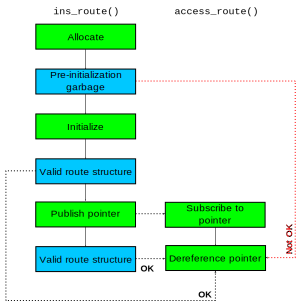
\includegraphics{defer/pubsub}}
\caption{Publication/Subscription Constraints}
\label{fig:defer:Publication/Subscription Constraints}
\end{figure}

Unfortunately, as laid out in
\cref{sec:toolsoftrade:Shared-Variable Shenanigans}
and reiterated in
\cref{sec:defer:Minimal Insertion and Deletion},
it is unwise to use \IXplx{plain access}{es} for these publication and subscription
operations.
It is instead necessary to inform both the compiler and the CPU
of the need for care, as can be seen from
\cref{fig:defer:Publication/Subscription Constraints},
which illustrates interactions between concurrent executions of
\co{ins_route()} (and its caller) and \co{read_gptr()} from
\cref{lst:defer:Insertion and Deletion With Concurrent Readers}.

The \co{ins_route()} column from
\cref{fig:defer:Publication/Subscription Constraints}
shows \co{ins_route()}'s caller allocating a new \co{route} structure,
which then contains pre-initialization garbage.
The caller then initializes the newly allocated structure, and then
invokes \co{ins_route()} to publish a pointer to the new \co{route}
structure.
Publication does not affect the contents of the structure, which
therefore remain valid after publication.

The \co{access_route()} column from this same figure shows
the pointer being subscribed to and dereferenced.
This dereference operation absolutely must see a valid \co{route}
structure rather than pre-initialization garbage because referencing
garbage could result in memory corruption, crashes, and hangs.
As noted earlier, avoiding such garbage means that the publish and
subscribe operations must inform both the compiler and the CPU of the
need to maintain the needed ordering.

Publication is carried out by \co{rcu_assign_pointer()}, which ensures that
\co{ins_route()}'s caller's initialization is ordered before the actual
publication operation's store of the pointer.
In addition, \co{rcu_assign_pointer()} must be atomic in the sense that 
concurrent readers see either the old value of the pointer or the new
value of the pointer, but not some mash-up of these two values.
These requirements are met by the C11 store-release operation, and in
fact in the Linux kernel, \co{rcu_assign_pointer()} is defined in terms
of \co{smp_store_release()}, which is similar to C11 store-release.

Note that if concurrent updates are required, some sort of synchronization
mechanism will be required to mediate among multiple concurrent
\co{rcu_assign_pointer()} calls on the same pointer.
In the Linux kernel, locking is the mechanism of choice, but pretty
much any synchronization mechanism may be used.
An example of a particularly lightweight synchronization mechanism is
\cref{chp:Data Ownership}'s data ownership:
If each pointer is owned by a particular thread, then that thread may
execute \co{rcu_assign_pointer()} on that pointer with no additional
synchronization overhead.

\QuickQuiz{
	Wouldn't use of data ownership for RCU updaters mean that
	the updates could use exactly the same sequence of instructions
	as would the corresponding single-threaded code?
}\QuickQuizAnswer{
	Sometimes, for example, on TSO systems such as x86 or the IBM
	mainframe where a store-release operation emits a single store
	instruction.
	However, weakly ordered systems must also emit a memory barrier
	or perhaps a store-release instruction.
	In addition, removing data requires quite a bit of additional
	work because it is necessary to wait for pre-existing readers
	before freeing the removed data.
}\QuickQuizEnd

Subscription is carried out by \co{rcu_dereference()}, which orders
the subscription operation's load from the pointer is before the
dereference.
Similar to \co{rcu_assign_pointer()}, \co{rcu_dereference()} must be
atomic in the sense that the value loaded must be that from a single
store, for example, the compiler must not tear the load.\footnote{
	That is, the compiler must not break the load into multiple
	smaller loads, as described under ``load tearing'' in
	\cref{sec:toolsoftrade:Shared-Variable Shenanigans}.}
Unfortunately, compiler support for \co{rcu_dereference()} is at best
a work in progress~\cite{PaulEMcKennneyConsumeP0190R4,PaulEMcKenney2017markconsumeP0462R1,JFBastien2018P0750R1consume}.
In the meantime, the Linux kernel relies on volatile loads, the details of
the various CPU architectures, coding
restrictions~\cite{PaulEMcKenney2014rcu-dereference},
and, on DEC Alpha~\cite{ALPHA2002}, a memory-barrier instruction.
However, on other architectures, \co{rcu_dereference()} typically
emits a single load instruction, just as would the equivalent single-threaded
code.
The coding restrictions are described in more detail in
\cref{sec:memorder:Address- and Data-Dependency Difficulties},
however, the common case of field selection (\qtco{->}) works quite well.
Software that does not require the ultimate in read-side performance
can instead use C11 acquire loads, which provide the needed ordering and
more, albeit at a cost.
It is hoped that lighter-weight compiler support for \co{rcu_dereference()}
will appear in due course.

In short, use of \co{rcu_assign_pointer()} for publishing pointers and
use of \co{rcu_dereference()} for subscribing to them successfully avoids the
``Not OK'' garbage loads depicted in
\cref{fig:defer:Publication/Subscription Constraints}.
These two primitives can therefore be used to add new data to linked
structures without disrupting concurrent readers.

\QuickQuiz{
	But suppose that updaters are adding and removing multiple data
	items from a linked list while a reader is iterating over that
	same list.
	Specifically, suppose that a list initially contains elements
	A, B, and C, and that an updater removes element A and then
	adds a new element D at the end of the list.
	The reader might well see \{A, B, C, D\}, when that sequence of
	elements never actually ever existed!
	In what alternate universe would that qualify as ``not disrupting
	concurrent readers''???
}\QuickQuizAnswer{
	In the universe where an iterating reader is only required to
	traverse elements that were present throughout the full duration
	of the iteration.
	In the example, that would be elements B and C\@.
	Because elements A and D were each present for only part of the
	iteration, the reader is permitted to iterate over them, but not
	obliged to.
	Note that this supports the common case where the reader is simply
	looking up a single item, and does not know or care about the
	presence or absence of other items.

	If stronger consistency is required, then higher-cost
	synchronization mechanisms are required, for example, sequence
	locking or reader-writer locking.
	But if stronger consistency is \emph{not} required (and it very often
	is not), then why pay the higher cost?
}\QuickQuizEnd

Adding data to a linked structure without disrupting readers is a good thing,
as are the cases where this can be done with no added read-side cost compared
to single-threaded readers.
However, in most cases it is also necessary to remove data, and this is the
subject of the next section.

\subsubsection{Wait For Pre-Existing RCU Readers}
\label{sec:defer:Wait For Pre-Existing RCU Readers}

In its most basic form, RCU is a way of waiting for things to finish.
Of course, there are a great many other ways of waiting for things to
finish, including reference counts, reader-writer locks, events, and so on.
The great advantage of RCU is that it can wait for each of
(say) 20,000 different things without having to explicitly
track each and every one of them, and without having to worry about
the performance degradation, scalability limitations, complex deadlock
scenarios, and memory-leak hazards that are inherent in schemes
using explicit tracking.

In RCU's case, each of the things waited on is called an
\emph{RCU read-side critical section}.
As hinted at in
\cref{sec:defer:Toy Implementation}, an RCU read-side critical
section starts with an \co{rcu_read_lock()} primitive, and ends with a
corresponding \co{rcu_read_unlock()} primitive.
RCU read-side critical sections can be nested, and may contain pretty
much any code, as long as that code does not contain a quiescent state,
for example, within the Linux kernel, it is illegal to sleep within
an RCU read-side critical section because a context switch is a quiescent
state.\footnote{
	However, a special form of RCU called SRCU~\cite{PaulEMcKenney2006c}
	does permit general sleeping in SRCU read-side critical sections.}
If you abide by these conventions, you can use RCU to wait for \emph{any}
pre-existing RCU read-side critical section to complete, and
\co{synchronize_rcu()} uses indirect means to do the actual
waiting~\cite{MathieuDesnoyers2012URCU,McKenney:2013:SDS:2483852.2483867}.

\begin{figure}
\centering
\resizebox{3in}{!}{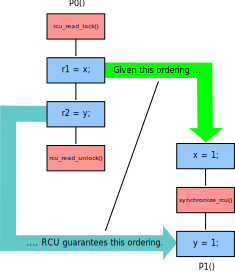
\includegraphics{defer/RCUGuaranteeFwd}}
\caption{RCU Reader and Later Grace Period}
\label{fig:defer:RCU Reader and Later Grace Period}
\end{figure}

The relationship between an RCU read-side critical section and a later
RCU grace period is an if-then relationship, as illustrated by
\cref{fig:defer:RCU Reader and Later Grace Period}.
If any portion of a given critical section precedes the beginning of
a given grace period, then RCU guarantees that all of that critical
section will precede the end of that grace period.
In the figure, \co{P0()}'s access to \co{x} precedes \co{P1()}'s access
to this same variable, and thus also precedes the grace period generated
by \co{P1()}'s call to \co{synchronize_rcu()}.
It is therefore guaranteed that \co{P0()}'s access to \co{y} will precede
\co{P1()}'s access.
In this case, if \co{r1}'s final value is 0, then \co{r2}'s final value
is guaranteed to also be 0.

\QuickQuiz{
	What other final values of \co{r1} and \co{r2} are possible in
	\cref{fig:defer:RCU Reader and Later Grace Period}?
}\QuickQuizAnswer{
	The \co{r1 == 0 && r2 == 0} possibility was called out in the text.
	Given that \co{r1 == 0} implies \co{r2 == 0}, we know that
	\co{r1 == 0 && r2 == 1} is forbidden.
	The following discussion will show that both
	\co{r1 == 1 && r2 == 1} and \co{r1 == 1 && r2 == 0} are possible.
}\QuickQuizEnd

\begin{figure}
\centering
\resizebox{3in}{!}{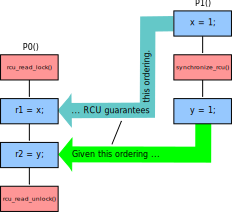
\includegraphics{defer/RCUGuaranteeRev}}
\caption{RCU Reader and Earlier Grace Period}
\label{fig:defer:RCU Reader and Earlier Grace Period}
\end{figure}

The relationship between an RCU read-side critical section and an earlier
RCU grace period is also an if-then relationship, as illustrated by
\cref{fig:defer:RCU Reader and Earlier Grace Period}.
If any portion of a given critical section follows the end of
a given grace period, then RCU guarantees that all of that critical
section will follow the beginning of that grace period.
In the figure, \co{P0()}'s access to \co{y} follows \co{P1()}'s access
to this same variable, and thus follows the grace period generated by
\co{P1()}'s call to \co{synchronize_rcu()}.
It is therefore guaranteed that \co{P0()}'s access to \co{x} will follow
\co{P1()}'s access.
In this case, if \co{r2}'s final value is 1, then \co{r1}'s final value
is guaranteed to also be 1.

\QuickQuiz{
	What would happen if the order of \co{P0()}'s two accesses was
	reversed in
	\cref{fig:defer:RCU Reader and Earlier Grace Period}?
}\QuickQuizAnswer{
	Absolutely nothing would change.
	The fact that \co{P0()}'s loads from \co{x} and \co{y} are
	in the same RCU read-side critical section suffices;
	their order is irrelevant.
}\QuickQuizEnd

\begin{figure}
\centering
\resizebox{3in}{!}{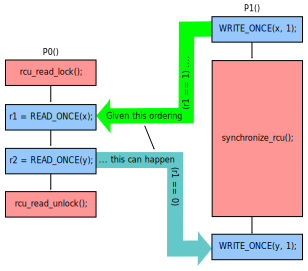
\includegraphics{defer/RCUGuaranteeMid}}
\caption{RCU Reader Within Grace Period}
\label{fig:defer:RCU Reader Within Grace Period}
\end{figure}

Finally, as shown in
\cref{fig:defer:RCU Reader Within Grace Period},
an RCU read-side critical section can be completely overlapped by
an RCU grace period.
In this case, \co{r1}'s final value is 1 and \co{r2}'s final value is 0.

However, it cannot be the case that \co{r1}'s final value is 0 and \co{r2}'s
final value is 1.
This would mean that an RCU read-side critical section had completely
overlapped a grace period, which is forbidden (or at the very least
constitutes a bug in RCU).
RCU's wait-for-readers guarantee therefore has two parts:
\begin{enumerate*}[(1)]
\item If any part of a given RCU read-side critical section precedes
the beginning of a given grace period, then the entirety of that
critical section precedes the end of that grace period.
\item If any part of a given RCU read-side critical section follows
the end of a given grace period, then the entirety of that
critical section follows the beginning of that grace period.
\end{enumerate*}
This definition is sufficient for almost all RCU-based algorithms, but
for those wanting more,
simple executable formal models of RCU are available
as part of Linux kernel v4.17 and later, as discussed in
\cref{sec:formal:Axiomatic Approaches and RCU}.
In addition, RCU's ordering properties are examined in much
greater detail in \cref{sec:memorder:RCU}.

\QuickQuiz{
	What would happen if \co{P0()}'s accesses in
	\crefrange{fig:defer:RCU Reader and Later Grace Period}{fig:defer:RCU Reader Within Grace Period}
	were stores?
}\QuickQuizAnswer{
	The exact same ordering rules would apply, that is,
	(1)~If any part of \co{P0()}'s RCU read-side critical section
	preceded the beginning of \co{P1()}'s grace period, all of
	\co{P0()}'s RCU read-side critical section would precede the
	end of \co{P1()}'s grace period, and
	(2)~If any part of \co{P0()}'s RCU read-side critical section
	followed the end of \co{P1()}'s grace period, all of \co{P0()}'s
	RCU read-side critical section would follow the beginning of
	\co{P1()}'s grace period.

	It might seem strange to have RCU read-side critical sections
	containing writes, but this capability is not only permitted,
	but also highly useful.
	For example, the Linux kernel frequently carries out an
	RCU-protected traversal of a linked data structure and then
	acquires a reference to the destination data element.
	Because this data element must not be freed in the meantime,
	that element's reference counter must necessarily be incremented
	within the traversal's RCU read-side critical section.
	However, that increment entails a write to memory.
	Therefore, it is a very good thing that memory writes are
	permitted within RCU read-side critical sections.

	If having writes in RCU read-side critical sections still seems
	strange, please review
	\cref{sec:count:Applying Exact Limit Counters},
	which presented a use case for writes in reader-writer locking
	read-side critical sections.
}\QuickQuizEnd

Although RCU's wait-for-readers capability really is sometimes used to
order the assignment of values to variables as shown in
\crefrange{fig:defer:RCU Reader and Later Grace Period}
{fig:defer:RCU Reader Within Grace Period},
it is more frequently used to safely free data elements removed from
a linked structure, as was done in
\cref{sec:defer:Introduction to RCU}.
The general process is illustrated by the following pseudocode:

\begin{enumerate}
\item	Make a change, for example, remove an element from a linked list.
\item	Wait for all pre-existing RCU read-side critical sections to
	completely finish (for example, by using
	\co{synchronize_rcu()}).
\item	Clean up, for example, free the element that was replaced above.
\end{enumerate}

\begin{figure}
\centering
\IfEbookSize{
\resizebox{2in}{!}{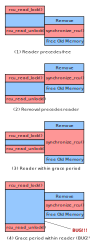
\includegraphics{defer/RCUGPorderingSummary}}
}{
\resizebox{2.5in}{!}{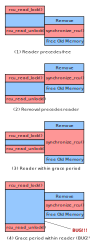
\includegraphics{defer/RCUGPorderingSummary}}
}
\caption{Summary of RCU Grace-Period Ordering Guarantees}
\label{fig:defer:Summary of RCU Grace-Period Ordering Guarantees}
\end{figure}

This more abstract procedure requires a more abstract diagram than
\crefrange{fig:defer:RCU Reader and Later Grace Period}
{fig:defer:RCU Reader Within Grace Period},
which are specific to a particular litmus test.
After all, an RCU implementation must work correctly regardless of
the form of the RCU updates and the RCU read-side critical sections.
\Cref{fig:defer:Summary of RCU Grace-Period Ordering Guarantees}
fills this need, showing the four possible scenarios, with time
advancing from top to bottom within each scenario.
Within each scenario, an RCU reader is represented by the left-hand
stack of boxes and RCU updater by the right-hand stack.

In the first scenario, the reader starts execution before the
updater starts the removal, so it is possible that this reader
has a reference to the removed data element.
Therefore, the updater must not free this element until after the
reader completes.
In the second scenario, the reader does not start execution until
after the removal has completed.
The reader cannot possibly obtain a reference to the already-removed
data element, so this element may be freed before the reader completes.
The third scenario is like the second, but illustrates that when the
reader cannot possibly obtain a reference to element, it is still
permissible to defer the freeing of that element until after the
reader completes.
In the fourth and final scenario, the reader starts execution before
the updater starts removing the data element, but this element
is (incorrectly) freed before the reader completed.
A correct RCU implementation will not allow this fourth scenario to
occur.
This diagram thus illustrates RCU's wait-for-readers functionality:
Given a grace period, each reader ends before the end of that grace
period, starts after the beginning of that grace period, or both, in
which case it is wholly contained within that grace period.

Because RCU readers can make forward progress while updates
are in progress, different readers might disagree about the state
of the data structure, a topic taken up by the next section.

\subsubsection{Maintain Multiple Versions of Recently Updated Objects}
\label{sec:defer:Maintain Multiple Versions of Recently Updated Objects}

This section discusses how RCU accommodates synchronization-free readers
by maintaining multiple versions of data.
Because these synchronization-free readers provide very weak temporal
synchronization, RCU users compensate via spatial synchronization.
Spatial synchronization was discussed in
\cref{cha:Partitioning and Synchronization Design}, and is heavily used
in practice to obtain good performance and scalability.
In this section, spatial synchronization will be used to attain a weak
(but useful) form of correctness as well as excellent performance and
scalability.

\Cref{fig:defer:Deletion With Concurrent Readers}
in
\cref{sec:defer:Minimal Insertion and Deletion}
showed a simple variant of spatial synchronization, in which different
readers running concurrently with \co{del_route()}
(see \cref{lst:defer:Insertion and Deletion With Concurrent Readers})
might see the old \co{route} structure or an empty list, but either
way get a valid result.
Of course, a closer look at
\cref{fig:defer:Insertion With Concurrent Readers}
shows that calls to \co{ins_route()} can also result in concurrent
readers seeing different versions:
Either the initial empty list or the newly inserted \co{route} structure.
Note that both reference counting
(\cref{sec:defer:Reference Counting})
and hazard pointers
(\cref{sec:defer:Hazard Pointers})
can also cause concurrent readers to see different versions, but
RCU's lightweight readers make this more likely.

\begin{figure}
\centering
\resizebox{3in}{!}{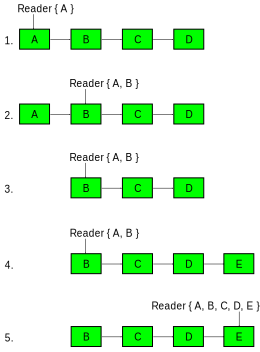
\includegraphics{defer/multver}}
\caption{Multiple RCU Data-Structure Versions}
\label{fig:defer:Multiple RCU Data-Structure Versions}
\end{figure}

However, maintaining multiple weakly consistent versions can provide
some surprises.
For example, consider
\cref{fig:defer:Multiple RCU Data-Structure Versions},
in which a reader is traversing a linked list that is concurrently
updated.\footnote{
	RCU linked-list APIs may be found in
	\cref{sec:defer:RCU Linux-Kernel API}.}
In the first row of the figure, the reader is referencing data item~A,
and in the second row, it advances to~B, having thus far seen A followed by~B\@.
In the third row, an updater removes element~A and in the fourth row
an updater adds element~E to the end of the list.
In the fifth and final row, the reader completes its traversal, having
seeing elements~A through~E\@.

Except that there was no time at which such a list existed.
This situation might be even more surprising than that shown in
\cref{fig:defer:Deletion With Concurrent Readers},
in which different concurrent readers see different versions.
In contrast, in
\cref{fig:defer:Multiple RCU Data-Structure Versions}
the reader sees a version that never actually existed!

One way to resolve this strange situation is via weaker semanitics.
A reader traversal must encounter any data item that was present
during the full traversal (B, C, and~D), and might or might not
encounter data items that were present for only part of the
traversal (A and~E).
Therefore, in this particular case, it is perfectly legitimate for
the reader traveral to encounter all five elements.
If this outcome is problematic, another way to resolve this situation is
through use of stronger synchronization mechanisms, such as reader-writer
locking, or clever use of timestamps and versioning.
The Linux kernel frequently uses sequence locking to provide tighter
consistency, as described in \cref{sec:together:Correlated Data Elements}.
Of course, stronger mechanisms will be more expensive, but then again
the engineering life is all about choices and tradeoffs.

Strange though this situation might seem, it is entirely consistent with
the real world.
As we saw in
\cref{sec:cpu:Overheads},
the finite speed of light cannot be ignored within a computer system,
and it most certainly cannot be ignored outside of this system.
This in turn means that any data within the system representing state
in the real world outside of the system is always and forever outdated,
and thus inconsistent with the real world.
Therefore, it is quite possible that the sequence \{A, B, C, D, E\}
occurred in the real world, but due to speed-of-light delays was
never represented in the computer system's memory.
In this case, the reader's surprising traversal would correctly reflect
reality.

As a result, algorithms operating on real-world data must account for
inconsistent data, either by tolerating inconsistencies or by taking
steps to exclude or reject them.
In many cases, these algorithms are also perfectly capable of dealing
with inconsistencies within the system.

The pre-BSD packet routing example laid out in
\cref{sec:defer:Running Example}
is a case in point.
The contents of a routing list is set by routing protocols, and these
protocols feature significant delays (seconds or even minutes) to avoid
routing instabilities.
Therefore, once a routing update reaches a given system,
it might well have been sending packets the wrong way for quite some time.
Sending a few more packets the wrong way for the few microseconds during
which the update is in flight is clearly not a problem because the same
higher-level protocol actions that deal with delayed routing updates
will also deal with internal inconsistencies.

Nor is Internet routing the only situation tolerating inconsistencies.
To repeat, any algorithm in which data within a system tracks
outside-of-system state must tolerate inconsistencies, which includes
security policies (often set by committees of humans), storage configuration,
and WiFi access points, to say nothing of removable hardware such as
microphones, headsets, cameras, mice, printers, and much else besides.
Furthermore, the large number of Linux-kernel RCU API uses shown in
\cref{fig:defer:RCU Usage in the Linux Kernel},
combined with the Linux kernel's heavy use of reference counting
and with increasing use of hazard pointers in other projects, demonstrates
that tolerance for such inconsistencies is more common than one might
imagine.

One root cause of this common-case tolerance of inconsistencies is
that single-item lookups are much more common in practice than are
full-data-structure traversals.
After all, full-data-structure traversals are much more expensive than
single-item lookups, so developers are motivated to avoid such traversals.
Not only are concurrent updates are less likely to affect a single-item
lookup than they are a full traversal, but it is also the case that an
isolated single-item lookup has no way of detecting such inconsistencies.
As a result, in the common case, such inconsistencies are not just
tolerable, they are in fact invisible.

In such cases, RCU readers can be considered to be fully ordered with
updaters, despite the fact that these readers might be executing the
exact same sequence of machine instructions that would be executed by
a single-threaded program.
For example, referring back to
\cref{lst:defer:Insertion and Deletion With Concurrent Readers}
on \cpageref{lst:defer:Insertion and Deletion With Concurrent Readers},
suppose that each reader thread invokes \co{access_route()} exactly
once during its lifetime, and that there is no other communication among
reader and updater threads.
\begin{fcvref}[ln:defer:Insertion and Deletion With Concurrent Readers]
Then each invocation of \co{access_route()} can be ordered after the
\co{ins_route()} invocation that produced the \co{route} structure
accessed by \clnref{access_rp} of the listing in \co{access_route()}
and ordered before any subsequent
\co{ins_route()} or \co{del_route()} invocation.
\end{fcvref}

In summary, maintaining multiple versions is exactly what enables the
extremely low overheads of RCU readers, and as noted earlier, many
algorithms are unfazed by multiple versions.
However, there are algorithms that absolutely cannot handle multiple versions.
There are techniques for adapting such algorithms to
RCU~\cite{PaulEdwardMcKenneyPhD}, for example, the use of sequence locking
described in \cref{sec:together:Correlated Data Elements}.

\paragraph{Exercises}
\label{sec:defer:Exercises}

These examples assumed that a mutex was held across the entire
update operation, which would mean that there could be at most two
versions of the list active at a given time.

\QuickQuizSeries{%
\QuickQuizB{
	How would you modify the deletion example to permit more than two
	versions of the list to be active?
}\QuickQuizAnswerB{
	One way of accomplishing this is as shown in
	\cref{lst:defer:Concurrent RCU Deletion}.

\begin{listing}
\begin{VerbatimL}
spin_lock(&mylock);
p = search(head, key);
if (p == NULL)
	spin_unlock(&mylock);
else {
	list_del_rcu(&p->list);
	spin_unlock(&mylock);
	synchronize_rcu();
	kfree(p);
}
\end{VerbatimL}
\caption{Concurrent RCU Deletion}
\label{lst:defer:Concurrent RCU Deletion}
\end{listing}

	Note that this means that multiple concurrent deletions might be
	waiting in \co{synchronize_rcu()}.
}\QuickQuizEndB
%
\QuickQuizE{
	How many RCU versions of a given list can be
	active at any given time?
}\QuickQuizAnswerE{
	That depends on the synchronization design.
	If a semaphore protecting the update is held across the grace period,
	then there can be at most two versions, the old and the new.

	However, suppose that only the search, the update, and the
	\co{list_replace_rcu()} were protected by a lock, so that
	the \co{synchronize_rcu()} was outside of that lock, similar
	to the code shown in
	\cref{lst:defer:Concurrent RCU Deletion}.
	Suppose further that a large number of threads undertook an
	RCU replacement at about the same time, and that readers
	are also constantly traversing the data structure.

	Then the following sequence of events could occur, starting from
	the end state of
	\cref{fig:defer:Multiple RCU Data-Structure Versions}:

	\begin{enumerate}
	\item	Thread~A traverses the list, obtaining a reference to
		Element~C.
	\item	Thread~B replaces Element~C with a new
		Element~F, then waits for its \co{synchronize_rcu()}
		call to return.
	\item	Thread~C traverses the list, obtaining a reference to
		Element~F.
	\item	Thread~D replaces Element~F with a new
		Element~G, then waits for its \co{synchronize_rcu()}
		call to return.
	\item	Thread~E traverses the list, obtaining a reference to
		Element~G.
	\item	Thread~F replaces Element~G with a new
		Element~H, then waits for its \co{synchronize_rcu()}
		call to return.
	\item	Thread~G traverses the list, obtaining a reference to
		Element~H.
	\item	And the previous two steps repeat quickly with additional
		new elements, so that all of them happen before any of
		the \co{synchronize_rcu()} calls return.
	\end{enumerate}

	Thus, there can be an arbitrary number of versions active,
	limited only by memory and by how many updates could be completed
	within a grace period.
	But please note that data structures that are updated so frequently
	are not likely to be good candidates for RCU\@.
	Nevertheless, RCU can handle high update rates when necessary.
}\QuickQuizEndE
}

\subsubsection{Summary of RCU Fundamentals}
\label{sec:defer:Summary of RCU Fundamentals}

This section has described the three fundamental components of RCU-based
algorithms:

\begin{enumerate}
\item	A publish-subscribe mechanism for adding new data,

\item	A way of waiting for pre-existing RCU readers to finish
	(see \cref{sec:memorder:RCU} for more detail),
	and

\item	A discipline of maintaining multiple versions to permit
	change without harming or unduly delaying concurrent RCU readers.
\end{enumerate}

\QuickQuiz{
	How can RCU updaters possibly delay RCU readers, given that
	neither \co{rcu_read_lock()} nor \co{rcu_read_unlock()}
	spin or block?
}\QuickQuizAnswer{
	The modifications undertaken by a given RCU updater will cause the
	corresponding CPU to invalidate cache lines containing the data,
	forcing the CPUs running concurrent RCU readers to incur expensive
	cache misses.
	(Can you design an algorithm that changes a data structure
	\emph{without}
	inflicting expensive cache misses on concurrent readers?
	On subsequent readers?)
}\QuickQuizEnd

These three RCU components allow data to be updated in face of concurrent
readers that might be executing the same sequence of machine instructions
that would be used by a reader in a single-threaded implementation.
These RCU components can be combined in different ways to implement a
surprising variety of different types of RCU-based algorithms.
However, it is usually better to work at higher levels of abstraction.
To this end, the next section describes the Linux-kernel API, which
includes simple data structures such as lists.
